\documentclass{beamer}
 
\usepackage[utf8]{inputenc}
\usepackage{epstopdf}
\usepackage{graphicx}
%Information to be included in the title page:
\title{Coordinate Geometry}
\subtitle{A Matrix approach}
\author{Gautham Gururajan \and Vignatha Vinjam}
\institute{Indian Institute of Technology Hyderabad}
\date{February 2019}
 
 
\begin{document}
 
\frame{\titlepage}
 
\begin{frame}
\frametitle{Problem}
A circle passes through the points $A = \begin{bmatrix} 2 & 3
\end{bmatrix}$ and $B = \begin{bmatrix} 4 & 5
\end{bmatrix}$
and it's Center lies on the line  
$ \begin{bmatrix}
-1 & 4
\end{bmatrix}\mathbf{x} + 3 = 0$.
\newline
\newline
\newline
Find the Radius of this Circle.

\end{frame}
\begin{frame}
\frametitle{Introduction}
The Given Problem can easily be solved using the following property:\newline \textit{The Perpendicular Bisector of a Chord Made by Joining Two Points on a Circle \textbf{\textit{Must}} pass through the Center of that Circle}
\end{frame}
\begin{frame}
\frametitle{Approach}
The steps we took to solve this problem were:
\begin{itemize}
 \item<1-> Use the Given Points to find a line passing through them.
 \item<2-> Find the midpoint of this chord.
 \item<3-> Calculate slope of the given chord, and thus calculate slope of it's perpendicular.
 \item<4-> Draw the line perpendicular to the chord, and passing through it's midpoint.
 \item<5-> Find the intersection of this perpendicular with the given line.
 \item<6-> Now that we have the center of the circle, calculate distance from either of the given points and thus obtain the radius.
\end{itemize}

\end{frame}

\begin{frame}
\frametitle{Solution}
\begin{itemize}
 \item<1-> We have $A = \begin{bmatrix} 2 & 3
 \end{bmatrix}$ and $B = \begin{bmatrix} 4 & 5
 \end{bmatrix}$ and the line : $ \begin{bmatrix}
 -1 & 4
 \end{bmatrix}\mathbf{x} + 3 = 0$. 
 \item<2-> C is the Midpoint of A-B, so : $C = (A+B)/2 = \begin{bmatrix} 3 & 4
 \end{bmatrix}$
 \item<3-> Through elementary operations, we see that the chord is represented by $\begin{bmatrix}
 -1 & 1 
 \end{bmatrix} \mathbf{x} - 1 = 0$
 \item<4-> The Perpendicular must thus be in the form of $\begin{bmatrix}
 1 & 1 
 \end{bmatrix} \mathbf{x} - k = 0$, with $C$ as the solution and on solving, we get $k = -7$
 \item<5-> Clearly, the Solution of the Given Line and this Perpendicular Bisector will give you the center of the circle. ie: \newline
 $\begin{bmatrix}
 1 & 1 \\
 -1 & 4 
 \end{bmatrix} \mathbf{x} = \begin{bmatrix}
 	-7 \\
 	 -3 
 \end{bmatrix}$
 \item<6-> $\mathbf{x} = \begin{bmatrix}
 	-7 \\
 	-3 
 \end{bmatrix}$$\begin{bmatrix}
1 & 1 \\
-1 & 4 
\end{bmatrix}^{-1}$

  
 
 
\end{itemize}

\end{frame}

\begin{frame}
\frametitle{Results}
From the Executed Python Program, we come to know that :
\begin{itemize}
\item<1->The Center of the Circle is : $\begin{bmatrix} 6.2 & 0.8
\end{bmatrix}$
\item<2-> The Radius of the Circle is : 4.741307836451879 units
\end{itemize}\textsl{}
\end{frame}

\begin{frame}
\frametitle{Plot}
\begin{figure}[h]
\centering
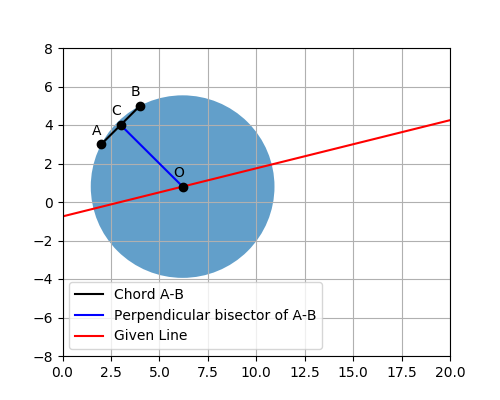
\includegraphics[scale=0.6]{/home/gautham/Desktop/EE1390_Project/Figures/Figure.png}
\caption{The Plotted Diagram of the lines meeting at the center of the circle}
\label{foobar-figure}
\end{figure}

\end{frame}

\end{document}

